\chapter{Methodology}
\label{chap:met}

\section{General Considerations}
\label{sec:general}
    The study of kin structures has its roots in the field of anthropology. Among the first foundational works was Henry Morgans'
    \textit{magnum opus} "Systems of Consanguinity and Affinity of the Human Family"\cite{morgan}, in which he argues that all human
    societies share a basic set of principles for social organization along kinship\footnote{Recall that in this thesis, the word
    "kinship" includes relatives as well as in-laws} lines, based on the principles of \textbf{consanguinity}
    (kinship by blood) and \textbf{affinity} (kinship by marriage). At the same time, he presented a sophisticated schema of social evolution
    based upon the relationship terms, the categories of kinship, used by peoples around the world. Through his analysis of kinship
    terms, Morgan discerned that the structure of the family and social institutions develop and change according to a specific
    sequence. He was the first to recognize and record six kin structures that are present in numerous societies and cultures around
    the world.

    Bearing in mind the vast variety of possible options, we are going to settle on just one specific kin structure, which we shall
    call \textit{traditional kinship}. We will devote the entire chapter to describing and modelling this structure.

    Following Henry Morgan, we recognize two primary types of family bonds: marital (affinity) and
    parental (consanguinity). These bonds define nine basic kin terms: \textit{father, mother, son, daughter, husband, wife, parent,
    child and spouse}. Observe that combining them in different ways will yield all possible kinship terms that can and do exist.
    For instance, \textit{cousin} is \textit{a child of a child of a parent of a parent} of a particular person. Another example:
    \textit{mother-in-law} is just \textit{a mother of a spouse}.

    Let us introduce several useful definitions:
    \begin{definition}
        We call a kinship term \textbf{abstract} iff it can refer to relatives of different sex. For instance, the word
        "parent" is an abstract kinship term, because it refers to a mother as well as to a father. Other well known examples:
        \textit{cousin, spouse, sibling} and \textit{child}.
    \end{definition}

    \begin{definition}
        In contrast, a \textbf{concrete} kin term refers only to relatives of the same sex, e.g. \textit{brother, aunt} and
        \textit{nephew}.
    \end{definition}

    \begin{definition}
        A \textbf{dyadic} kin term express the relationship between individuals as they relate to one another symmetrically, e.g. if I
        am your cousin (sibling), then you are also my cousin (sibling). The few, and uncommon, English dyadic terms involve in-laws:
        \textit{co-mothers-in-law, co-fathers-in-law, co-brothers-in-law, co-sisters-in-law, co-grandmothers}, and
        \textit{co-grandfathers}.
    \end{definition}

    \begin{definition}
        An \textbf{ego} is a focal point of a genealogy, i.e. it is a person from whose point of view we will describe all other
        people using kin terms.
    \end{definition}

    Now let us represent a traditional christian family tree as a special type of \textit{ontology} with its' own concepts,
    attributes, relations and constraints. Concepts are people in a family, their attributes are: \textit{name, birth date,
    birthplace, sex} and relations are parental and marital bonds with a wedding date.

    Together with the everything stated above, we have the following cultural constraints imposed on our genealogy:
    \begin{enumerate}
        \label{en:req}
        \item{Each person can have any finite number of children.}
        \item{Each person can have at most two parents of different sex.}
        \item{Each person can have at most one spouse of different sex.}
        \item{A spouse cannot be a \textit{direct relative}, i.e. a sibling or a parent. In other words, direct incest is
            prohibited.}
    \end{enumerate}

    When considering those prerequisites one should bear in mind that we deliberately focused only on rules, taboos and
    customs of one particular culture, namely American culture in the sense of Read \cite{read}. Under different assumptions and
    in further studies, these conditions can be relaxed and revisited.

    Apart from these four, here are two additional temporal constraints that express the interrelation between birth and wedding
    dates:
    \begin{enumerate}
        \item{No one can marry a person before he or she was born, i.e. a wedding date can only be strictly after a
            birth date of each spouse.}
        \item{A parent is born strictly before all of his (her) children.}
    \end{enumerate}
    Due to the general nature of these two constraints, they are always true in every genealogy and therefore can be safely
    assumed in our work.

    Every genealogy that meets these six requirements we shall call a \textbf{traditional family tree}. As the name "tree" suggests,
    we can indeed view this structure as a graph with its vertices as people and edges as bonds. Observe that every kinship term
    corresponds exactly to a \textit{path} between ego and specified relative. Under such a view, kin term becomes a set of instructions,
    telling how to get from the starting vertex \texttt{A} to the end vertex \texttt{B}. For example, consider the term
    \textit{mother-in-law}. What is it if not precisely a \textit{directive}: "firstly, go to my spouse, then proceed to her mother".
    The wonderful thing is that, due to the nature of kinship terminology, we can \textit{compose} them together to create
    new terms, even those which do not have their own name. This simple observation that we can see kinship terms as paths in a family
    tree underpins our entire thesis.

    Now, if we want to efficiently query a traditional family tree, we need to further investigate the mathematical features of
    the language of kinship terms. In the next sections we explore a formal model of kinship language, its syntax and semantics.
    Then we conclude this chapter with an examination of various approaches of tackling the concept of time. We also discuss
    possible augmentations to our model and the problem of \textit{term reduction}.

\section{Formal Language of Kinship}
\label{sec:formal}
    Here we present our attempt to model the language of traditional American, in the sense of Read\cite{read}, kinship terminology.
    There are three main characteristics that define every formal language: its syntax (spelling, how words are formed), semantics
    (what does particular word mean) and pragmatics (how a language is used). In order to describe it we must expound the first two.

    \subsection{Syntax}
    We use Backus-Naur Form to designate the syntax for our formal language. Let $\Sigma$ be the set of six basic kinship terms:
    \textit{father, mother, son, daughter, husband, wife}. Then we can express the grammar as follows:
    \begin{align*}
    \label{al:syntax}
    term ::= \Sigma | (term \cdot term) | (term \vee term) | (term)^{-1} | (term)^{\dagger}
    \end{align*}
    The first operation is called \textit{concatenation}, second -- \textit{fork}, third -- \textit{inverse} and the last --
    \textit{dual}. We denote this language by $\mathcal{L}$.

    Here are some examples of ordinary kinship terms expressed in our new language. Note that we deliberately omit superfluous
    parentheses and the composition sign for the sake of simplicity:
    \begin{itemize}
        \item{ Parent is $father \vee mother$. }
        \item{ Child is $son \vee daughter$. }
        \item{ Brother is $son (father \vee mother)$. }
        \item{ Sibling is $(son \vee daughter)(father \vee mother)$. }
        \item{ Uncle is $son(father \vee mother)(father \vee mother)$. }
        \item{ Daughter-in-law is $daughter \cdot husband$ }
        \item{ Co-mother-in-law is $mother(husband \vee wife)(son \vee daughter)$ }
    \end{itemize}
    From these examples you can see the real power of this language -- the power to express all possible used as well as not used
    kinship terms that can and do exist. Now the important step towards solving our main goal, developing a language for managing
    temporal genealogies, is to assign meaning to these words. From now on we distinguish between \textit{artificial} kinship terms,
    i.e. well-formed terms of our formalization, and \textit{natural} kin terms used in ordinary English. By referring to just terms,
    we mean the former, if nothing else is stated.

    \subsection{Semantics}
    Let $\Sigma^*$ stand for the set of all possible kin terms generated from the basis $\Sigma$ using the previously defined syntax.
    Let $\mathcal{G} = (V, E)$ be a traditional family tree with $V$ as a set of its vertices (people) and $E$ as a set of its
    edges (bonds). Moreover, because $\mathcal{G}$ is traditional, every person from the set $V$ have the following attributes:
    \begin{itemize}
        \item{A father. We will denote him as $father(p)$, a function that returns a \textit{set} containing at most one element.}
        \item{A mother. We will denote her by $mother(p)$.}
        \item{A set of his or her children: $children(p)$.}
        \item{A set of his or her sons: \[son(p) = \{c | c \in children(p) \land Male(p)\}\]}
        \item{A set of his or her daughters: \[daughter(p) = \{c | c \in children(p) \land Female(p)\}\]}
        \item{A spouse: $spouse(p)$.}
        \item{A husband: \[husband(p) = \{s | spouse(s) \land Male(p)\}\]}
        \item{A wife: \[wife(p) = \{s | spouse(s) \land Female(p)\}\]}
    \label{it:basic-func}
    \end{itemize}
    Due to the constraints stated in \ref{en:req}, result-set of $father$, $mother$, $spouse$, $husband$ and $wife$ can contain at
    most one element.

    Now we are ready to introduce \textbf{Denotational Semantics} for $\Sigma^*$. This name was chosen because it highly resembles
    namesake semantics of programming languages. Note that we regard kinship terms as \textit{functions} on subsets of $V$. Each
    function takes and returns a specific subset of all relatives, so its type is $f : \mathcal{P}(V) \to \mathcal{P}(V)$.

    We proceed by induction on the syntactic structure of $\mathcal{L}$. Let $t$ be an element of $\Sigma^*$, then:
    \begin{enumerate}
        \item{If $t \in \Sigma$, then $\llbracket t \rrbracket = F(t)$, where $F(t)$ assigns to each basic kin term its corresponding
            function from the list \ref{it:basic-func}.}
        \item{Term concatenation is a composition of two functions:
            \[\llbracket (t_1 \cdot t_2) \rrbracket = \llbracket t_1 \rrbracket \circ \llbracket t_2 \rrbracket\]}
        \item{Fork is a set-theoretic union of results of its sub-functions:
            \[\llbracket (t_1 \vee t_2) \rrbracket = p \mapsto \llbracket t_1 \rrbracket(p) \cup \llbracket t_2
        \rrbracket(p)\]}
        \item{Term inverse is exactly the inverse of its function:
            \[\llbracket t_1^{-1} \rrbracket = \llbracket t_1 \rrbracket^{-1}\]}
    \end{enumerate}
    The \textit{dual} operator ($\dagger$) is more difficult to define. We want it to mean exactly the same as the term, where the
    gender of each its basic sub-term is reversed, e.g. dual of "uncle" is "aunt", dual of "brother" is "sister" and so on.
    Here we can use induction once again:
    \begin{enumerate}
        \item{If $t \in \Sigma$, then $\llbracket t \rrbracket = D(t)$, where $D(t)$ is a basic term of opposite sex.}
        \item{Dual is distributive over concatenation, i.e. dual of concatenation is a concatenation of duals:
            \[\llbracket (t_1 \cdot t_2)^\dagger \rrbracket = \llbracket (t_1^\dagger \cdot t_1^\dagger) \rrbracket\]}
        \item{Dual is distributive over forking:
            \[\llbracket (t_1 \vee t_2)^\dagger \rrbracket = \llbracket (t_1^\dagger \vee t_2^\dagger ) \rrbracket\]}
        \item{Inverse commutes with dual:
                \[\llbracket (t^{-1})^{\dagger} \rrbracket = \llbracket (t^{\dagger})^{-1} \rrbracket\]}
    \end{enumerate}
    Observe that we also have the distributivity of concatenation over forking.
    This semantics allows us to efficiently navigate any family tree.

\section{Term Reduction}
\label{sec:reduc}
    Our artificial language has a problem: its too verbose. Indeed, to encode such ubiquitous kin terms as "uncle" or "great-nephew" one
    must use quite lengthy phrases that are hard to write and read. It is therefore important to have some sort of reduction mechanism
    for our language that will shorten long terms into a small set of common kinship relations to aid their understanding by a user.

    Firstly, let us analyse the problem. We have the following mapping $\omega$ between $\Sigma^*$ and the set of English kinship terms
    $\mathcal{W}$
    \begin{align*}
        son(father \vee mother) &\mapsto \text{brother}\\
        daughter(father \vee mother) &\mapsto \text{sister}\\
        father(father \vee mother) &\mapsto \text{grandfather}\\
        mother(father \vee mother) &\mapsto \text{grandmother}\\
        son(son \vee daughter) &\mapsto \text{grandson}\\
        \vdots\\
        father(son \vee daughter)(wife \vee husband)(son \vee daughter) &\mapsto \text{co-father-in-law}
    \end{align*}
    This dictionary allows us to effectively translate between kin terms of our artificial language $\mathcal{L}$ and their usual
    English equivalents. We can also view this mapping as a \textit{regular grammar} in the sense of Chomsky hierarchy\cite{chomsky}.
    However, note that we strictly prohibit mixing these two collections and therefore we deliberately avoid
    using words from the RHS in the LHS, because otherwise the grammar will lose its regularity and become \textit{at least}
    context-free, making the problem even more challenging. Let us define another function on top of $\omega$ that will replace the
    first sub-term $u \subset t$ in a term $t \in \Sigma^*$:
    \begin{align*}
        \Omega_u(t) = t[u / \omega(u)]
    \end{align*}
    Here the only change in meaning of $t[u / \omega(u)]$ is that the substitution takes place only once.

    Now the task can be stated thusly: given a term $t \in \Sigma^*$ find its shortest (in terms of the number of concatenations)
    translation under $\Omega$, i.e. which sub-terms need to be replaced and in what order.

    This problem can be easily reduced to that of of finding the desired point in the tree of all possible
    substitutions. Moreover, this point is actually a \textit{leaf}, because otherwise it is not the shortest one. But the latter
    can be solved by just searching for this leaf in-depth. Unfortunately, the search space grows exponentially with the
    number of entries in the dictionary $\omega$, thus making the naive brute-force approach unfeasible.

    Here we propose a heuristic greedy algorithm \ref{algo:red} that, although does not work for all cases, provides an expedient
    solution to the reduction problem in $O(n^2)$ time. Firstly, it finds the longest sub-term $u$ that exists in the dictionary
    $\omega$, then divides the term into two parts: left and right from $u$, after that it applies itself recursively to them, and
    finally it concatenates all three sub-terms together.

    Now let's analyse the time complexity of this algorithm:
    \begin{theorem}
        The execution time of the algorithm listed in \ref{algo:red} belongs to $\Theta(n^2)$.
    \end{theorem}
    \begin{proof}
        Let $T(n)$ be the execution time of the algorithm, where $n$ stands for the number of concatenations in a kin term.
        First of all, observe that $T(n)$ obeys the following recurrence:
        \begin{align}
            T(n) = 2 T(n / 2) + O(n^2)
        \end{align}
        Indeed, we make a recursive call exactly \textit{two} times and each call receives roughly the half of the specified term.
        During execution the function passes through two nested cycles, so one call costs us $O(n^2)$.

        Secondly, we use the \textbf{Master Method} from the famous book \textit{Introduction to Algorithms}\cite{cormen} by Cormen et al.
        In our case $a = 2$, $b = 2$, and $f(n) = O(n^2)$. Observe, that if we take $\epsilon$ to be any positive real number below
        one: $0 < \epsilon < 1$, then $f(n) = \Omega(n^{\log_ba + \epsilon}) = \Omega(n^{1 + \epsilon})$.

        Let us show that $f(n)$ satisfies the \textit{regularity} criterion: $af(n / b) \leqslant cf(n)$ for some constant $c < 1$.
        Indeed, just pick $c = 1/2$:
        \begin{align*}
            2f(n / 2) &\leqslant cf(n),\\
            2\frac{n^2}{4} &\leqslant cn^2,\\
            \frac{1}{2}n^2 &\leqslant cn^2,\\
            \frac{1}{2}n^2 &\leqslant \frac{1}{2}n^2
        \end{align*}
        Thus, we can use the third case from the Master Method, which tells us that $T(n) = \Theta(n^2)$.
    \end{proof}

    \subsection{Pursuing Confluence}
    Current approach listed in \ref{algo:red} has one major disadvantage: like any other greedy algorithm it can fail to choose a
    correct reduction path between two terms with equal amount of concatenations.
    We can alleviate this by augmenting our rewriting system, based on $\omega$ dictionary, with a feature called \textit{confluence},
    also known as \textit{Church-Rosser} property:
    \begin{definition}
        An abstract term rewriting system is said to possess \textbf{confluence}, if, when two terms $N$ and $P$ can be yielded from $M$,
        then they can be reduced to the single term $Q$. Figure \ref{fig:conf} depicts this scenario.
    \end{definition}
    Not only we can fix our reduction algorithm by introducing this property, but also we can improve the time complexity, making it
    linear.

    \begin{figure}
        \centering
        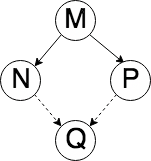
\includegraphics[width=0.2\linewidth]{figs/confluence.png}
        \caption{Confluence in a term rewriting system.}
        \label{fig:conf}
    \end{figure}

    One way to achieve confluence is to attach a single kinship term to any possible path in a family tree.
    Observe, that English kinship terms have a specific pattern that we can exploit. All relatives who are distant enough from ego
    have the following structure of their kin term:
    \begin{align*}
        n^{th} \text{ cousin } m^{th} \text{ times removed}
    \end{align*}
    In-laws also have their own pattern, where the ending "-in-law" is appended to a valid consanguine kinship term. However, this
    applies only to people, who are linked together by only one nuptial bond. For instance, there is no single term for a husband of
    ego's wife's sister. These relations can be accounted for by \textit{prefixing} "-in-law" with an ordinal, which shows the number
    of marital bonds that one should pass in order to go to such person. Under this representation, last example will receive the term
    "brother
    \textit{twice}-in-law". Generalizing that scheme we will get a pattern that looks like the following:
    \begin{align*}
        \langle \text{Consanguine kinship term} \rangle k^{th} \text{ times-in-law}
    \end{align*}

    We can also view this as an attribution of a distinct \textit{natural number} to every vertex with ego as an \textit{offset}, thus
    imposing a natural ordering on the set of all vertices. This assignment can be made in such a way that reducing a kinship term $n$
    will correspond \textit{exactly} to the calculation of $n$ from some arithmetic expression like $5 \cdot (2 + 3) + 4$, thus
    providing a \textbf{translation} between the language of all valid arithmetic expressions and our formal language of kinship
    $\mathcal{L}$.

    However, it is not the topic of this thesis, so we are leaving it to the considerations of future researches.

\section{Incorporating Time}
    Now the only matter that is left to address is an adequate representation of time. Historically, there are two main approaches
    for modelling time: point-based and interval-based. The former treats time as a single continuous line with distinguished points
    as specific \textit{events}, and the latter uses \textit{segments} of that line to represent time entries, which is more famous.
    For instance, it was used in Allen's interval algebra\cite{allen}. For the sake of simplicity we chose the former approach,
    because it can easily imitate intervals by treating them as endpoints of a line segment.

    Not only we want to talk about different events by modelling them as points on a line, but also we want to orient ourselves on
    that line, i.e. to know where we are, which events took place in the past and which will happen in the future. Thus, we need to
    select exactly one point that will stand for the present moment and call it "now". Then all point to the left will be in the past,
    and all point to the right will be in the future. Also, notice that any set with total ordering on it will suffice, because the
    continuous nature of a line is redundant in point-based model. Collecting everything together, we have the following formalisation
    of time:
    \begin{align*}
        \mathcal{M} = \langle T, now, \leqslant \rangle
    \end{align*}
    Where $T$ is a non-empty set with arbitrary elements, $now \in T$, and $\leqslant$ is a total ordering relation on $T$.

    Within this model we can reason about which event comes \textit{before} or \textit{after}, what events took place in the past or
    in the future, and so on.

    When considering family trees it is necessary to define only five predicates:
    \begin{enumerate}
        \item{$Before(x, y)$ is true iff $x < y$.}
        \item{$After(x, y)$ is true iff $x > y$.}
        \item{$During(x, s, f)$ is true iff $s \leqslant x \leqslant f$.}
        \item{$Past(x)$ is true iff $Before(x, now)$.}
        \item{$Future(x)$ is true iff $After(x, now)$.}
    \end{enumerate}
    Those relations are the basis from which all other operations on $\mathcal{M}$ can be defined. It is also interesting to note
    that, since any ordering relation generates a \textit{topology} over its structure, we can speak about time in terms of its
    topological properties.

    This observation concludes our methodology chapter.
